\vspace{-5pt}
\section{A Case Study of Cross-point ReRAM Macro Design}\label{sec:macro}
Since the array size of a cross-point ReRAM array is limited by
the reliability requirements, the design of a ReRAM macro is different
from the traditional DRAM design. 
%A cross-point ReRAM macro is implemented
%by connecting a number of small cross-point arrays with
%appropriate peripheral circuity and organizations. 
In this section, we evaluate the area, energy consumption, and bandwidth of a
256 Mbits ReRAM macro.
We use an organization similar to Kawahara's design~\cite{crossbar_Panasonic}, where
%We apply the similar memory organization as Kawahara's
%work~\cite{crossbar_Panasonic}. 
a 256 Mbits ReRAM macro is divided into 
eight planes. Each 32~Mbit plane has separate wordline
decoder, bitline selectors, sense amplifiers, and write circuity. Due to
space constraints, we present results for only
four typical cell parameters: ($Kr=20,
I_w=40uA$), ($Kr=20, I_w=200uA$), ($Kr=40, I_w=40uA$), and ($Kr=40,
I_w=200uA$). For each of them, we vary the number of bit per write to
investigate the relation among the area, energy consumption, and bandwidth
of the ReRAM macro.


%Figure~\ref{fig:aaable}
Table~II shows the total area, energy consumption, and bandwidth of the
256 Mbits ReRAM macro. Consistent with our earlier discussion, 
as the device nonlinearity improves, both area and energy 
goes down. The only downside is the noise margin restriction
imposed for reads. Similarly, as the drive current increases, the overhead
goes up due to large wordline drivers and bitline multiplexors. 
In summary, it is clear that increased bandwidth comes at the cost of area
and energy. 

To better understand the ideal design choice for a given device parameter,
we investigated three metrics: bandwidth per
nanojoule ($BW/nJ$), bandwidth per square millimeter($BW/mm^2$), and
bandwidth per nanojoule per square millimeter ($BW/(nJ\cdot mm^2)$).
Figure~\ref{fig:BWpAE}~(a) shows how $BW/mm^2$ scale as we increase the 
number of bits modified per write operation. From the figure, for a given
energy budget, writing one bit at a time provides at least~48\% better bandwidth 
compared to the best performing muti-bit writes. Hence, with the right choice
of global interconnect, interleaving writes across multiple sub-arrays is
an interesting design point. 
With multi-bit writes, as the number of bits per write increases, the energy
efficiency also increases. However, as the word size increases, the voltage
drop in the array also increases, which needs to be compensated by increasing
the operating voltage of the array (Section~\ref{sec:w_and_r}). Beyond 32~bits, this
increase in voltage, outweighing the bandwidth improvement, effectively reducing
the energy efficiency.
Thus from energy standpoint, multi-bit write is optimal when the word size is
8-32~bits, depending upon the nonlinearity and drive current. 
Figure~\ref{fig:BWpAE}~(b) shows the effect of multi-bit writes on bandwidth per
square millimeter. Unlike energy, as long as the drive current is less, 
it is beneficial to increase the word size as much as possible to improve
bandwidth for a given area. Also, writing one bit at a time is the least 
attractive option for a design primarily constrained by the area.
Figure~\ref{fig:BWpAE2} takes into account both energy and area, and 
provides a ``sweet spot'' for multi-bit writes.
Thus by understanding the key characteristics of cross-point array, we can 
identify an optimal configuration that best meets the design constrains. 

%Bandwidth per nanojoule reflects the energy efficiency on the bandwidth.
%The higher the bandwidth and the less amount of energy used to achieve a
%larger values of this metric. Besides, since the area is directly related
%to the cost, bandwidth per square millimeter is a good indicator of the
%economics of the bandwidth. As shown in Figure~\ref{fig:BWpAE} the
%bandwidth per nanojoule for single-bit write is always better than that
%for multi-bit write operation. Besides, there also exist a optimal number
%of bits per write for multi-bit write schemes: 32 bits for the cell with
%Kr=20, and 8 bits for cells with Kr=40. However, from the bandwidth per
%square millimeter point of view, the cells with different write current
%have different situation: for cells with large write current
%($I_w=200uA$), optimal number of bits per write is 16 bits. On the other
%hand, if the write current scales to $40uA$, the bandwidth per square
%millimeter increases monotonically with the increase of write bit number,
%and the large number of bit per write is favorable. The reason for this
%different is that, for the cell with large write current, the wordline
%drivers and bitline multiplexors can no longer be hidden underneath the
%array, which impact the area efficiency of the entire macro.
%Figure~\ref{fig:BWpAE2} shows the bandwidth per nanojoule per square
%millimeter results. Similarly, this metric also has a optimal number of
%bits per write for different cells: 8 bits for the cell with Kr=20, and 4
%bits for cells with Kr=40. However, we should note that, even for the same
%ReRAM cell, the ``sweet spot'' for different metric is different.
%Therefore, we can conclude that the optimal configuration varies with the
%optimization target($BW/nJ$, $BW/mm^2$, or $BW/(nJ\cdot mm^2)$).

%\begin{figure}[!t]
%\centering\label{fig:aaable}
%  % Requires \usepackage{graphicx}
%  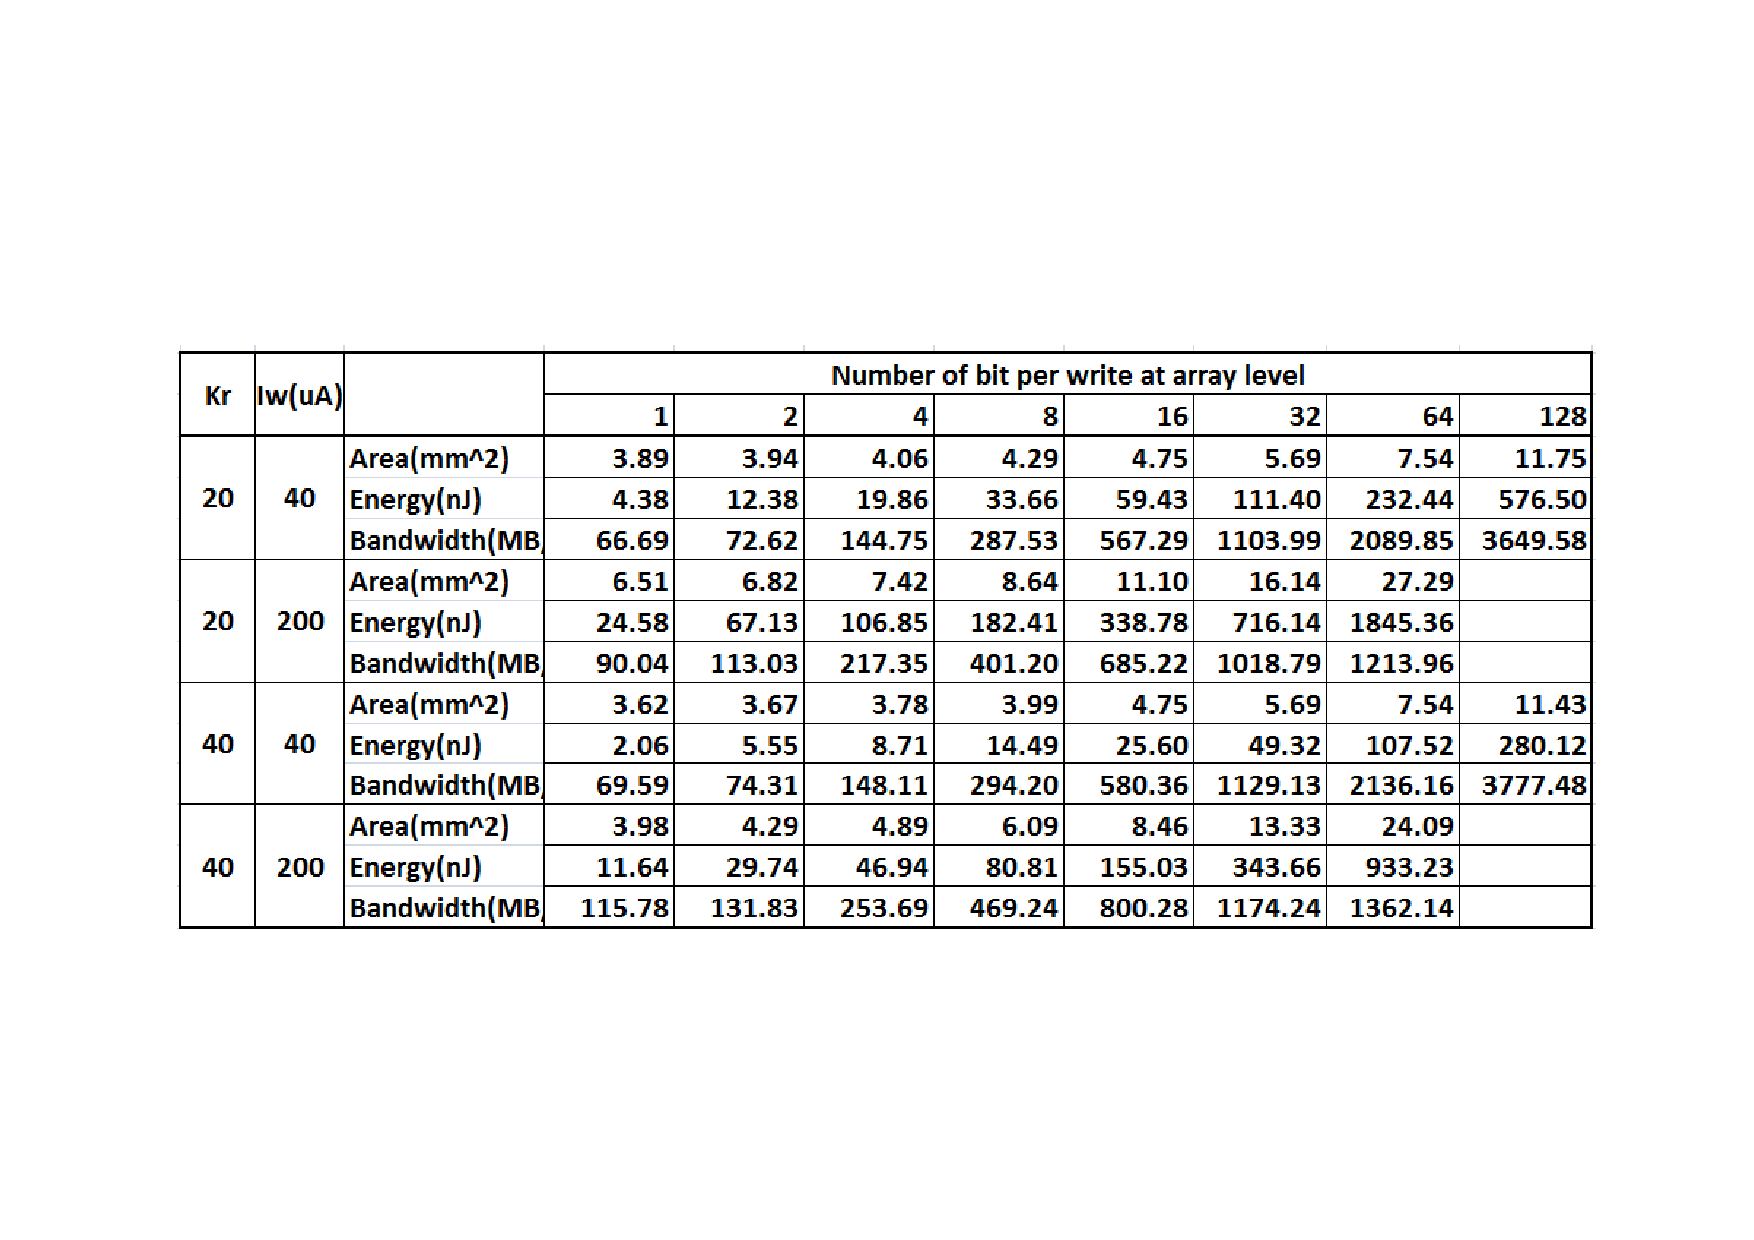
\includegraphics[width=0.5\textwidth]{./figures/Table}\\
%  \caption{Area, energy, and bandwidth results of 256 Mbits ReRAM macro.}
%  \vspace{-5pt}
%\end{figure}


%\begin{figure}[!]
%\centering\label{fig:EpJ}
%  % Requires \usepackage{graphicx}
%  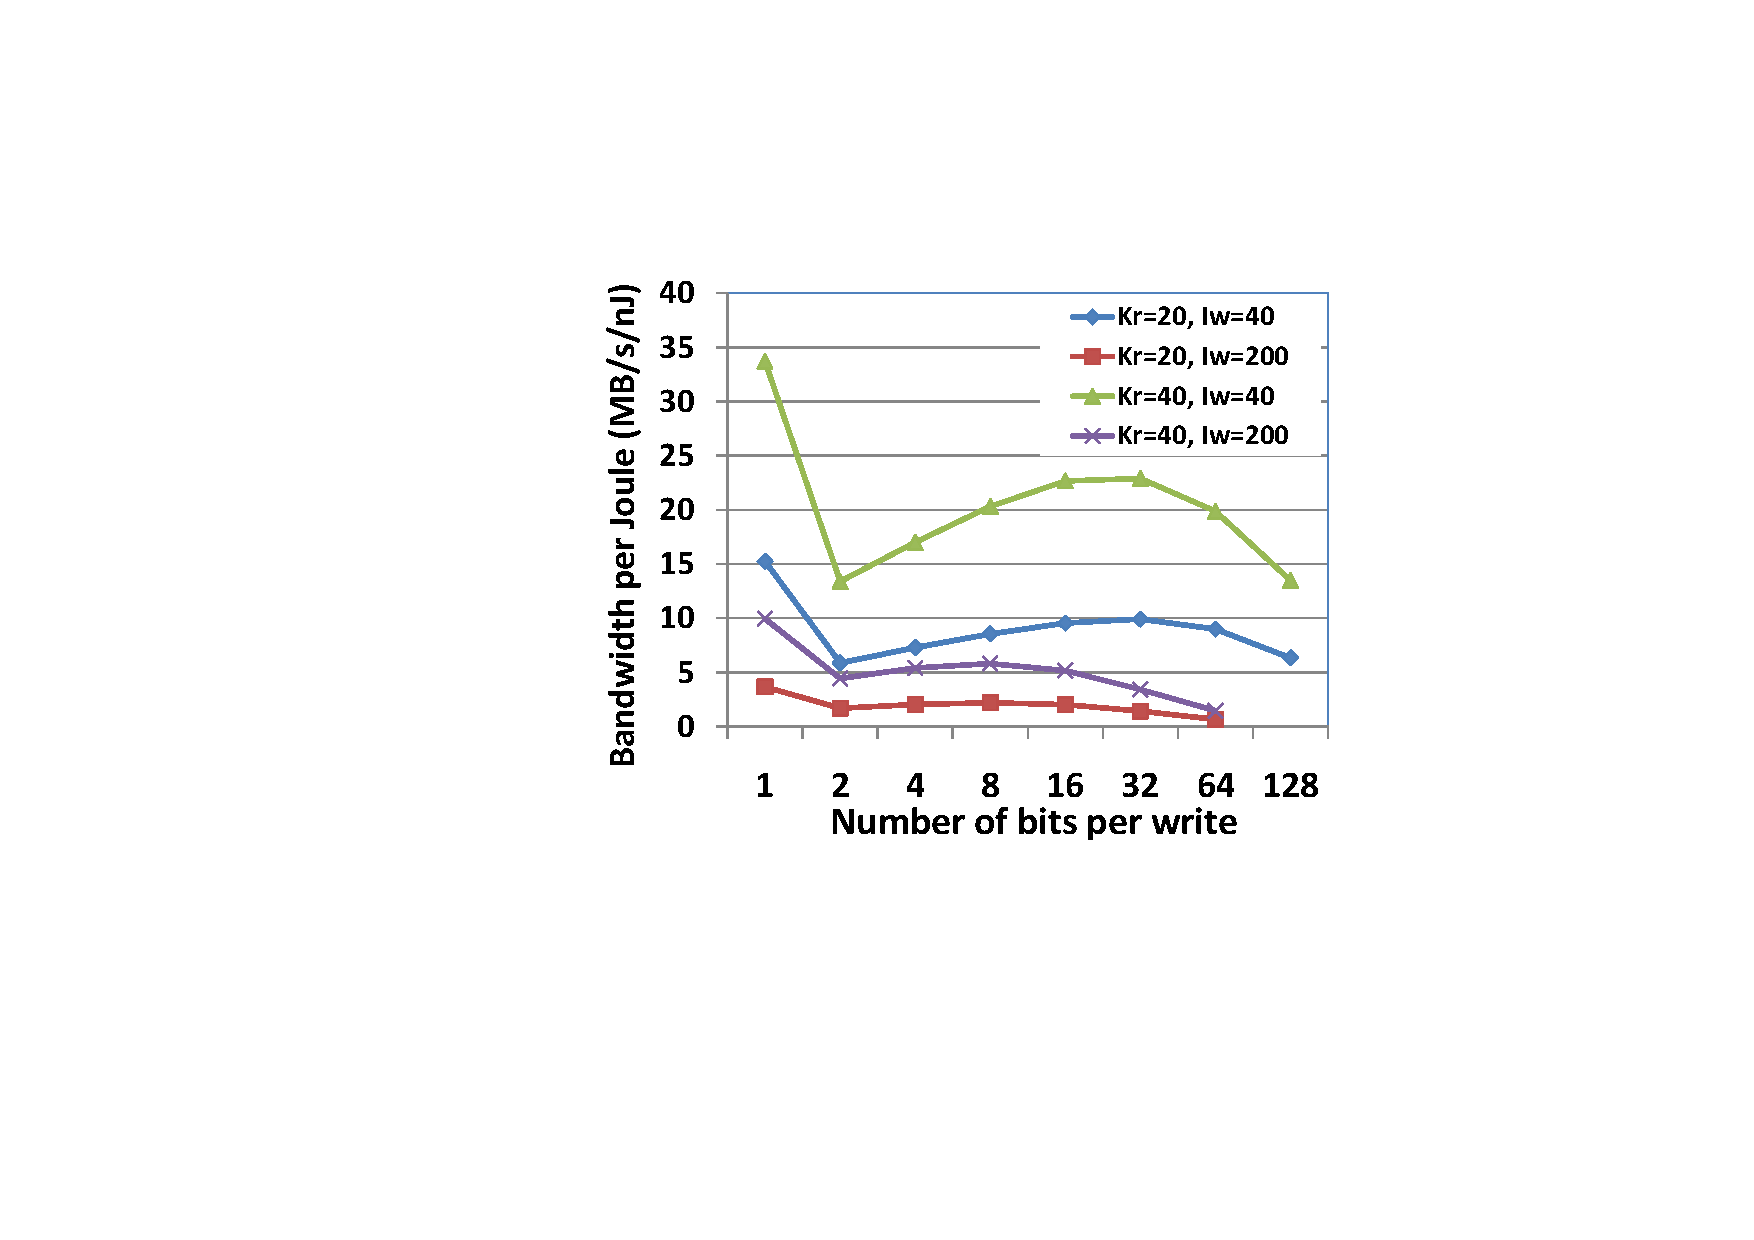
\includegraphics[width=2.3 in]{./figures/EpJ2}\\
%  \caption{Bandwidth-per-Joule of 256 Mbits ReRAM macro.}
%  \vspace{-15pt}
%\end{figure}


\begin{figure}[!]
\centering\label{fig:BWpAE}
  % Requires \usepackage{graphicx}
  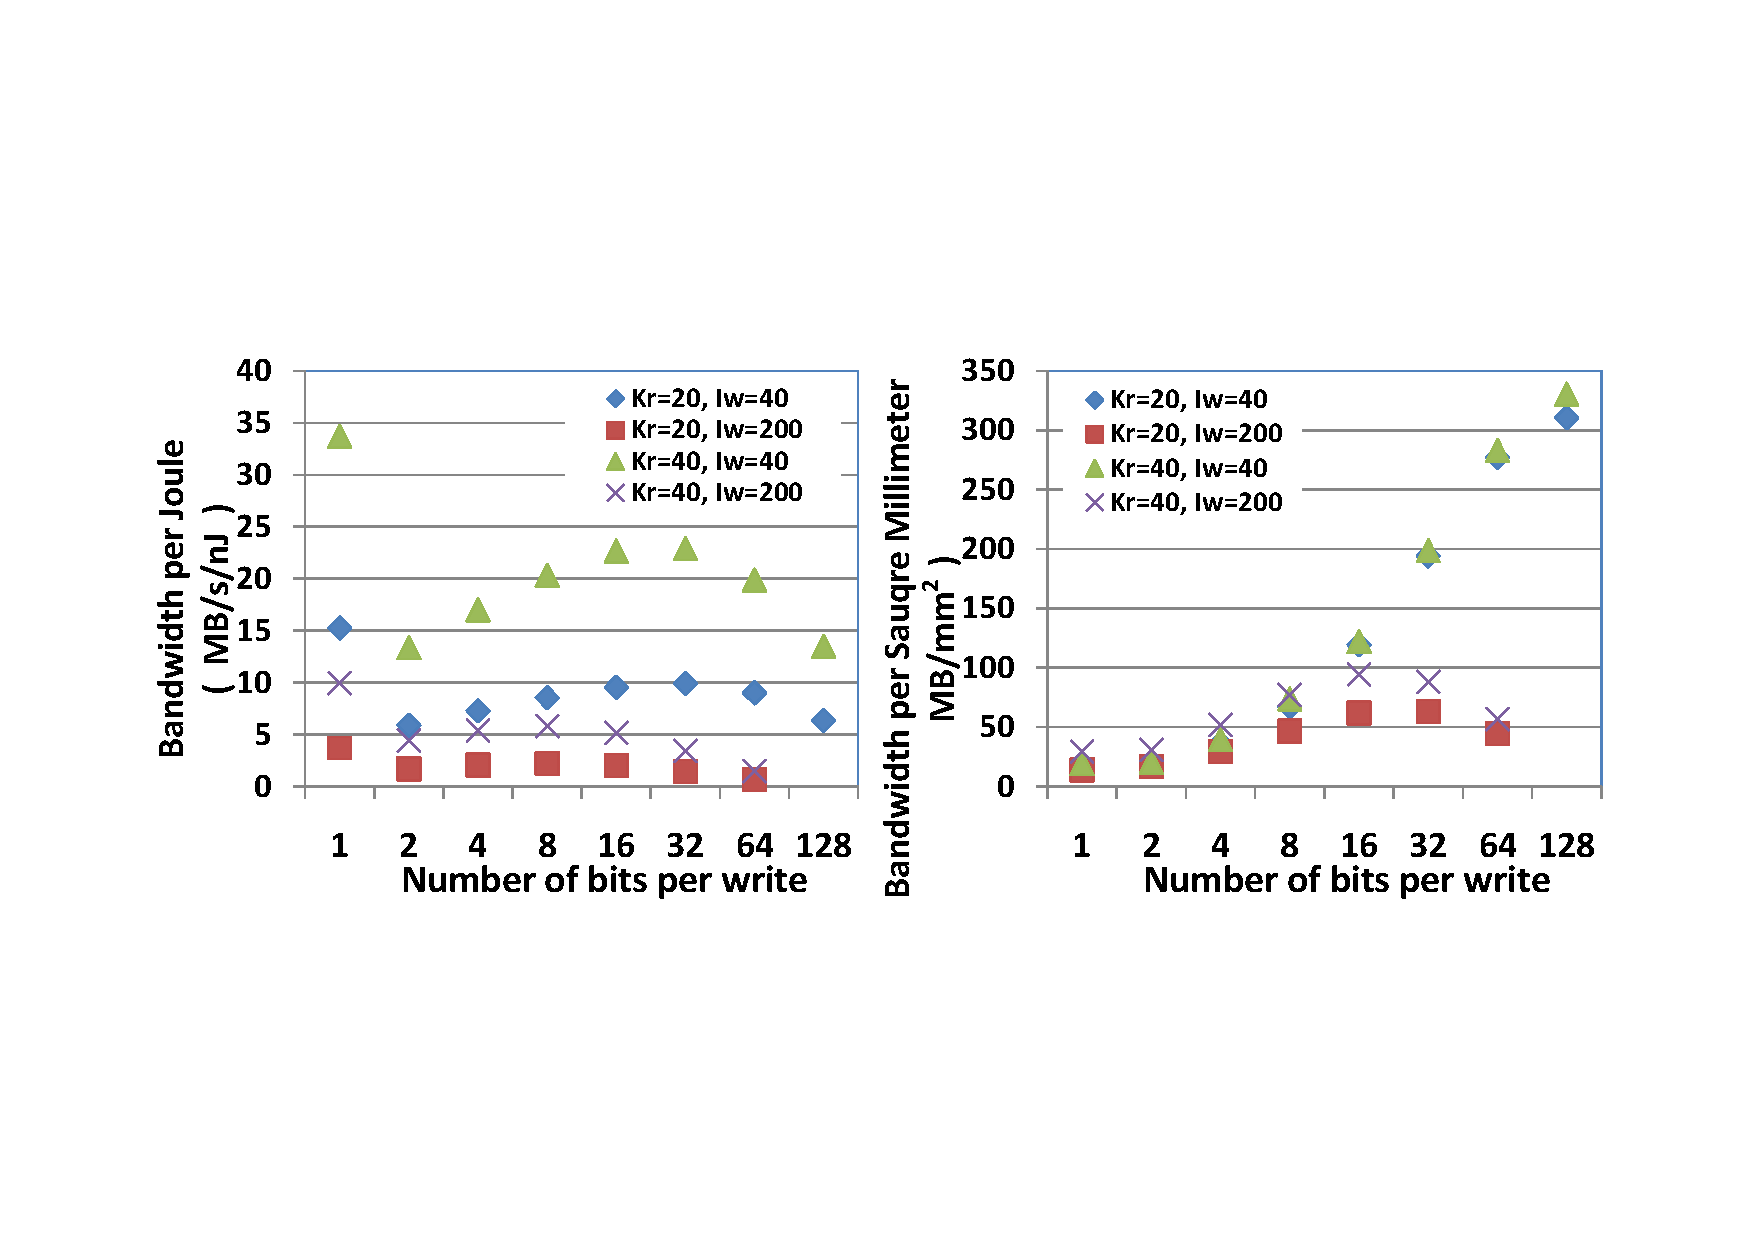
\includegraphics[width=3.4 in]{./figures/BWpAE}\\
  \caption{Bandwidth-per-Joule of 256 Mbits ReRAM macro.}
  \vspace{-5pt}
\end{figure}
\begin{figure}[!]
\centering\label{fig:BWpAE2}
  % Requires \usepackage{graphicx}
  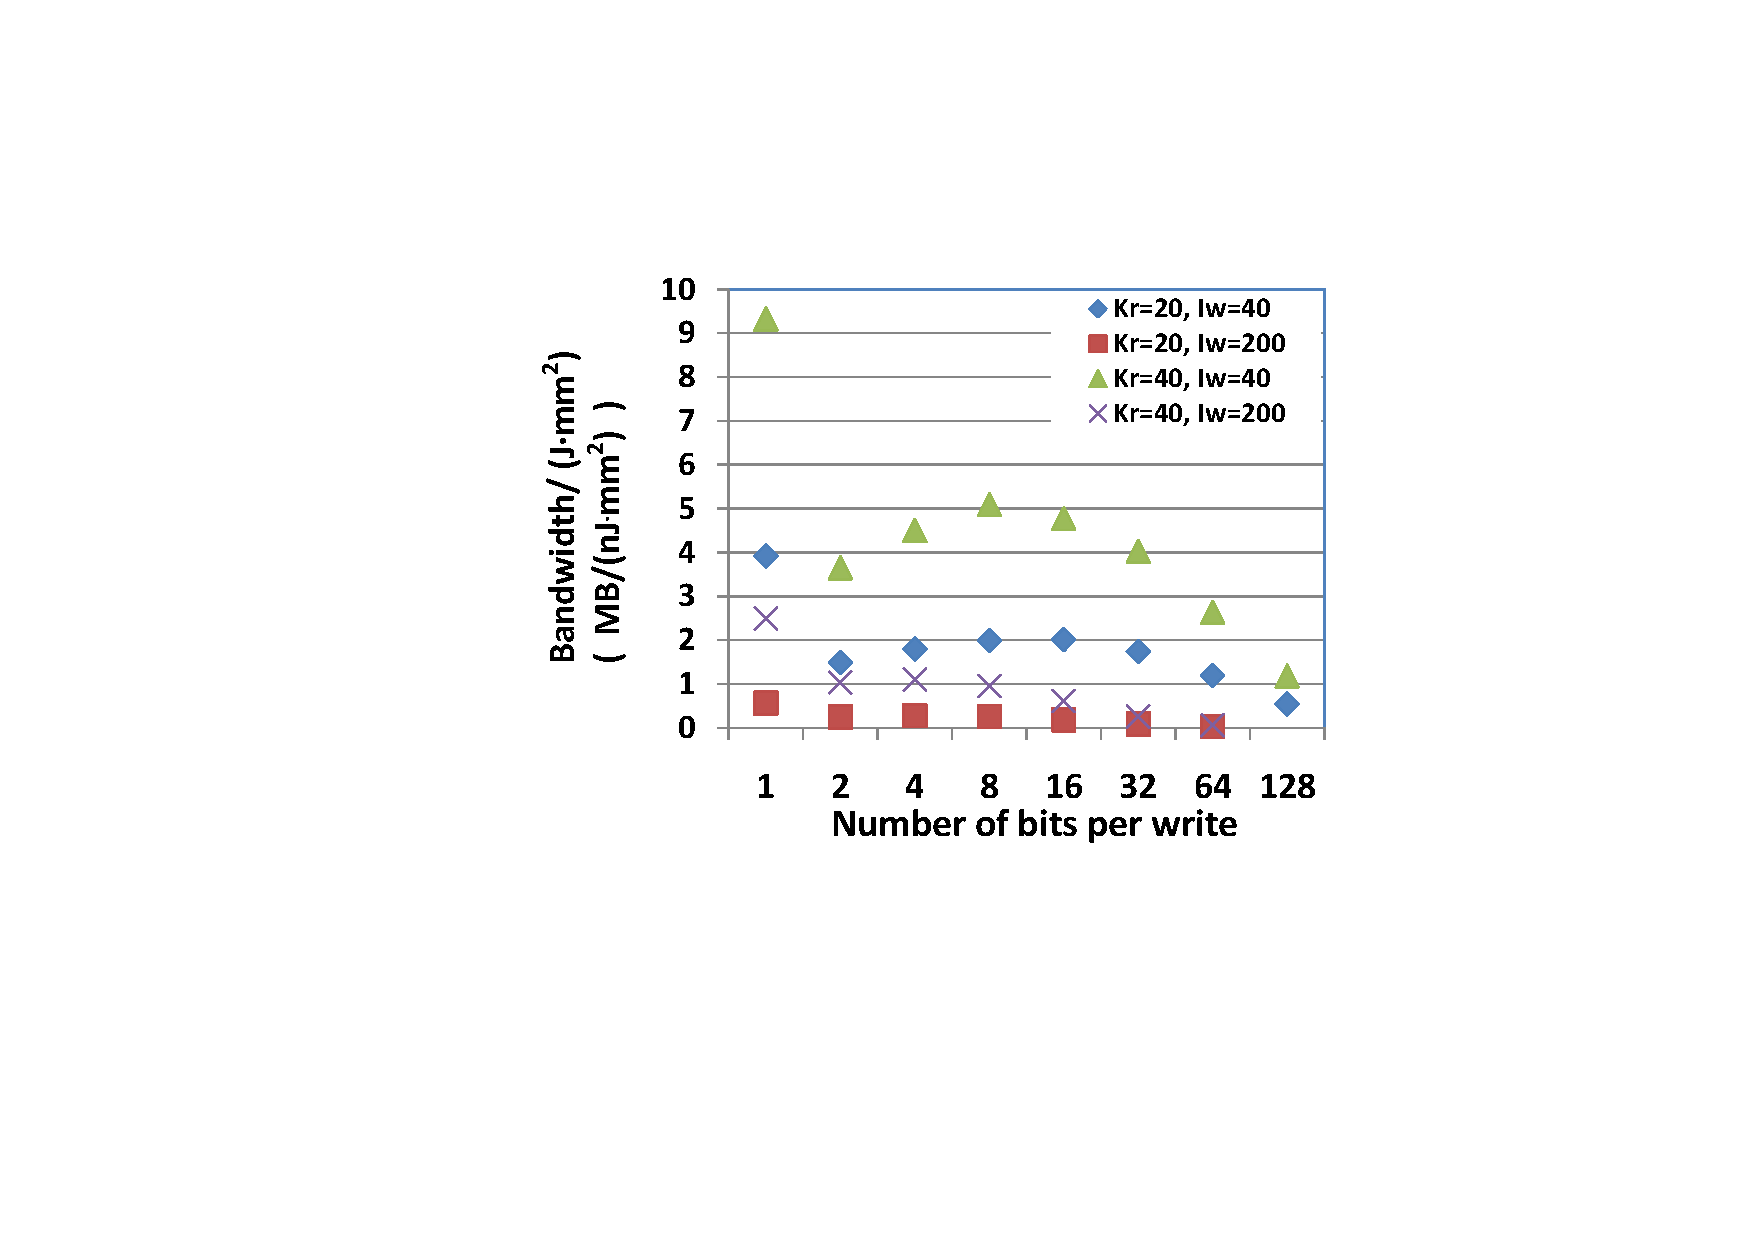
\includegraphics[width=2 in]{./figures/BWpAE2}\\
  \caption{Bandwidth-per-Joule of 256 Mbits ReRAM macro.}
  \vspace{-15pt}
\end{figure}
